%----------------------------------------------------------------------
% Problem 3

\begingroup
\allowdisplaybreaks

\newpage
\section{Problem 3}

\textbf{Exercise 3 in Section 4.10}

\subsection{Solution}

The model operator $G$ and noisy data vector $\bv{d}_n$ are provided in \verb|crosswell.mat|. The problem also provides depths for the sources and receivers, and a standard deviation of $\sigma = 0.5 \unit{\milli\second}$. The model operator and data are scaled by the standard deviation to form a weighted least squares solution. 

\begin{align*}
	W = \sigma I,\,\,\,G_w = W G,\,\,\,\bv{d}_w = W \bv{d}_n
\end{align*}

The model operator $G \in\R^{256 \times 256}$ where both $m = n = 256$. The rank of $G$ is $243$, which implies that $G_w$ is rank-deficient. The model operator is visualized in figure \ref{fig: prob3 model operator G_w}.

\begin{figure}[h] 
	\centering
	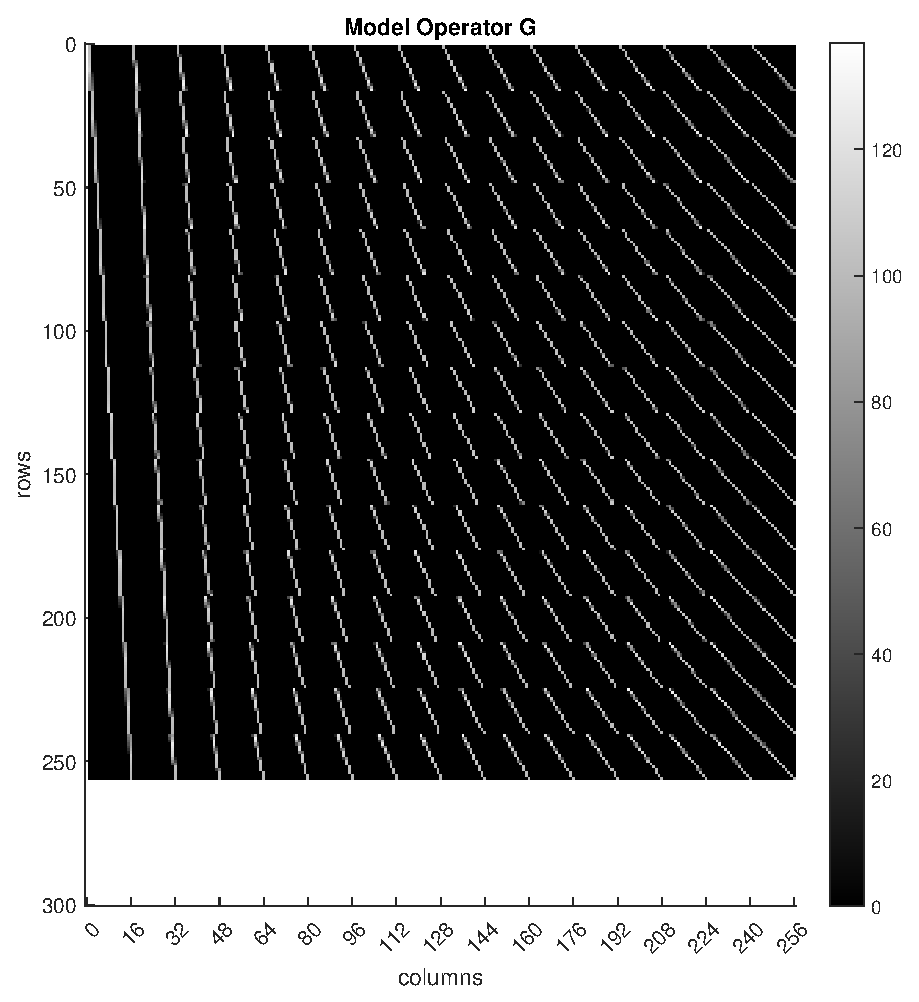
\includegraphics[width=0.65\textwidth]{./images/prob3_model_operator_G.eps}
	\caption{Model Operator $G_w$}
	\label{fig: prob3 model operator G_w}
\end{figure}
\FloatBarrier


% Part A
\subsubsection{Part A - Inverse Problem Solution via TSVD}

The L-curve was created using the provided functions \verb*|l_curve_tsvd()| and \verb*|l_curve_corner()| in the \verb*|PEIP| library. The inputs to the functions used the provided values of $G$ and $\bv{d}$, not their weighted versions. This resulted in the following plot in figure \ref{fig: prob3 partA L-curve}, where the reported truncated value $p' = 58$.

 \begin{figure}[h] 
 	\centering
 	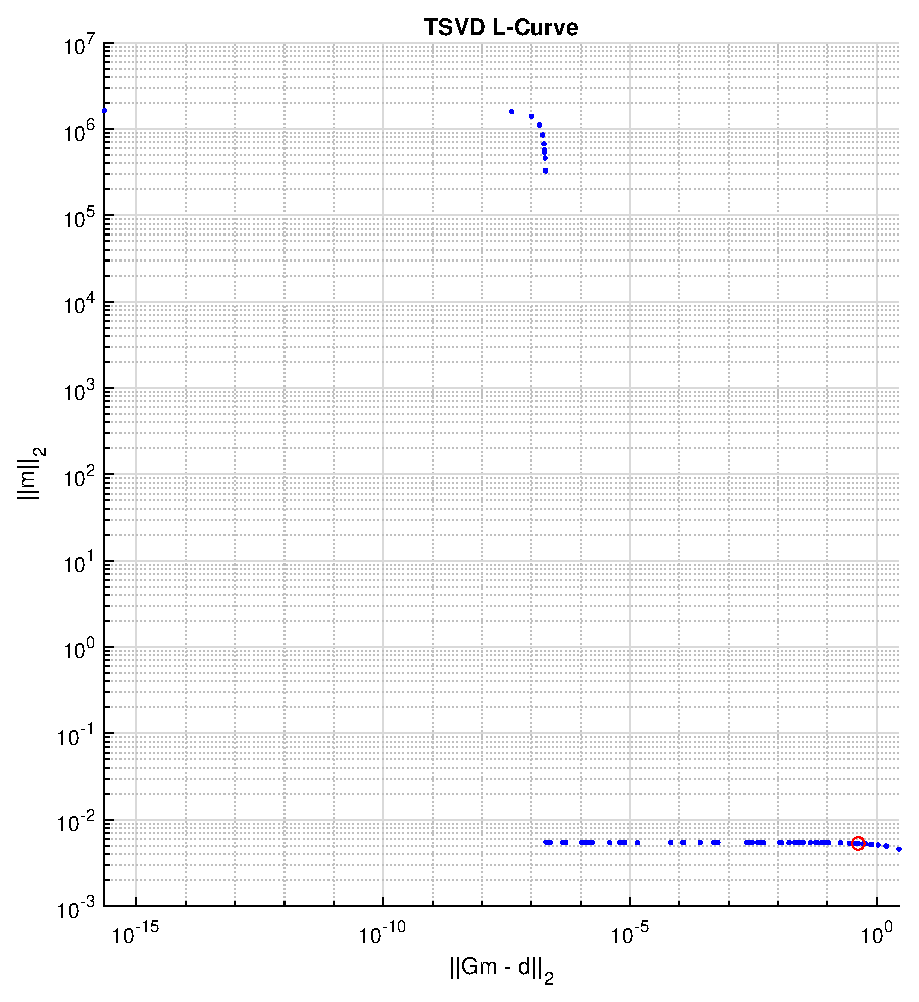
\includegraphics[width=0.85\textwidth]{./images/prob3_partA_TSVD_L_Curve.eps}
 	\caption{TSVD L-Curve}
 	\label{fig: prob3 partA L-curve}
 \end{figure}
 \FloatBarrier
 
 The model was solved using these generalized inverse where the SVD was re-computed using $G_w$. Truncating the generalized inverse solution to 58 singular values leads to the following model visualized in \ref{fig: prob3 partA model}.
 
  \begin{figure}[h] 
 	\centering
 	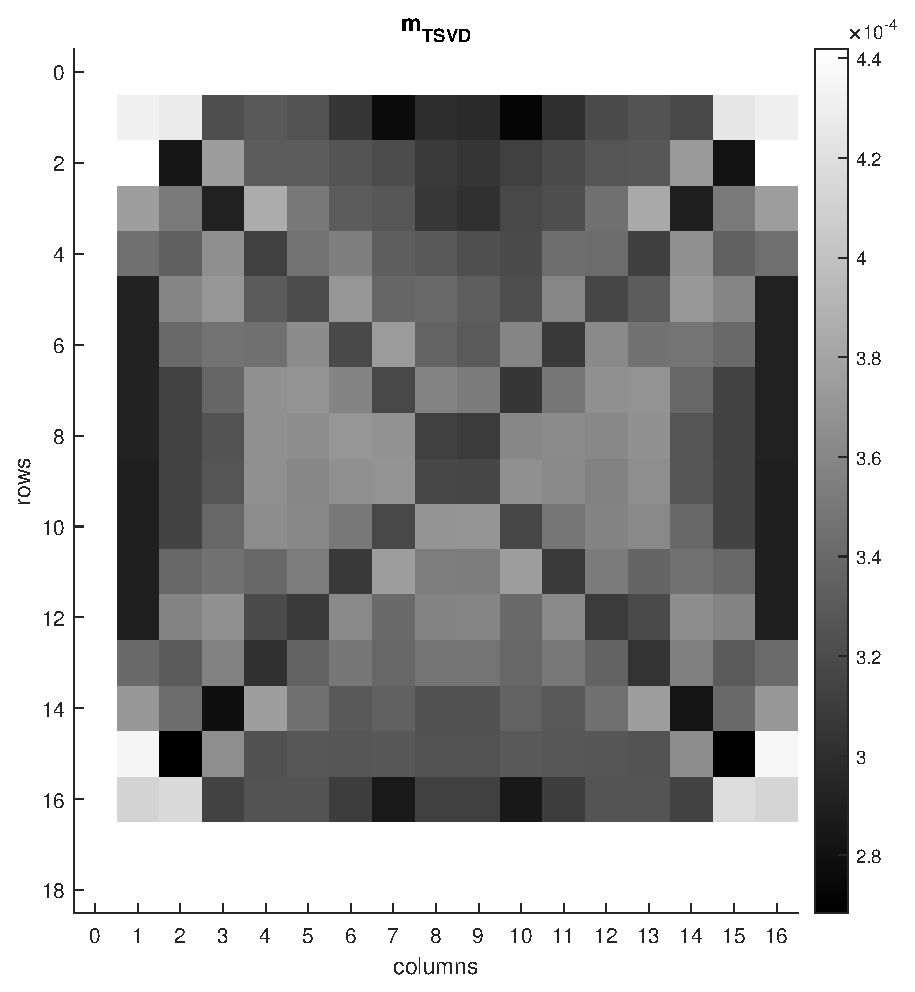
\includegraphics[width=0.85\textwidth]{./images/prob3_partA_m_tsvd.eps}
 	\caption{TSVD Solution}
 	\label{fig: prob3 partA model}
 \end{figure}
 \FloatBarrier
 
 
 % Part B
 \subsubsection{Part B - Inverse Problem Solution via Zeroth-Order Tikhonov Regularization}
 
 Again, the L-curve was created using the provided functions \verb*|l_curve_tikh_svd()| and \verb*|l_curve_corner()| in the \verb*|PEIP| library. The inputs to the functions used the provided values of $G$ and $\bv{d}$, not their weighted versions. This resulted in the following plot in figure \ref{fig: prob3 partB L-curve}, where the reported value $\alpha = 4.117 \times 10^{-7}$.
 
 \begin{figure}[h] 
 	\centering
 	\includegraphics[width=0.85\textwidth]{./images/prob3_partB_tikh_L_Curve.eps}
 	\caption{Zeroth-Order Tikhonov Regularization L-Curve}
 	\label{fig: prob3 partB L-curve}
 \end{figure}
 \FloatBarrier
 
The model was solved with the modified normal equations below.

\begin{align*}
	\bv{m}_{tikh} = \left(G_w^T G_w + \alpha^2 I\right)^{-1} G_w^T \bv{d}
\end{align*}

The result is provided in figure \ref{fig: prob3 partB model}.
 
 \begin{figure}[h] 
 	\centering
 	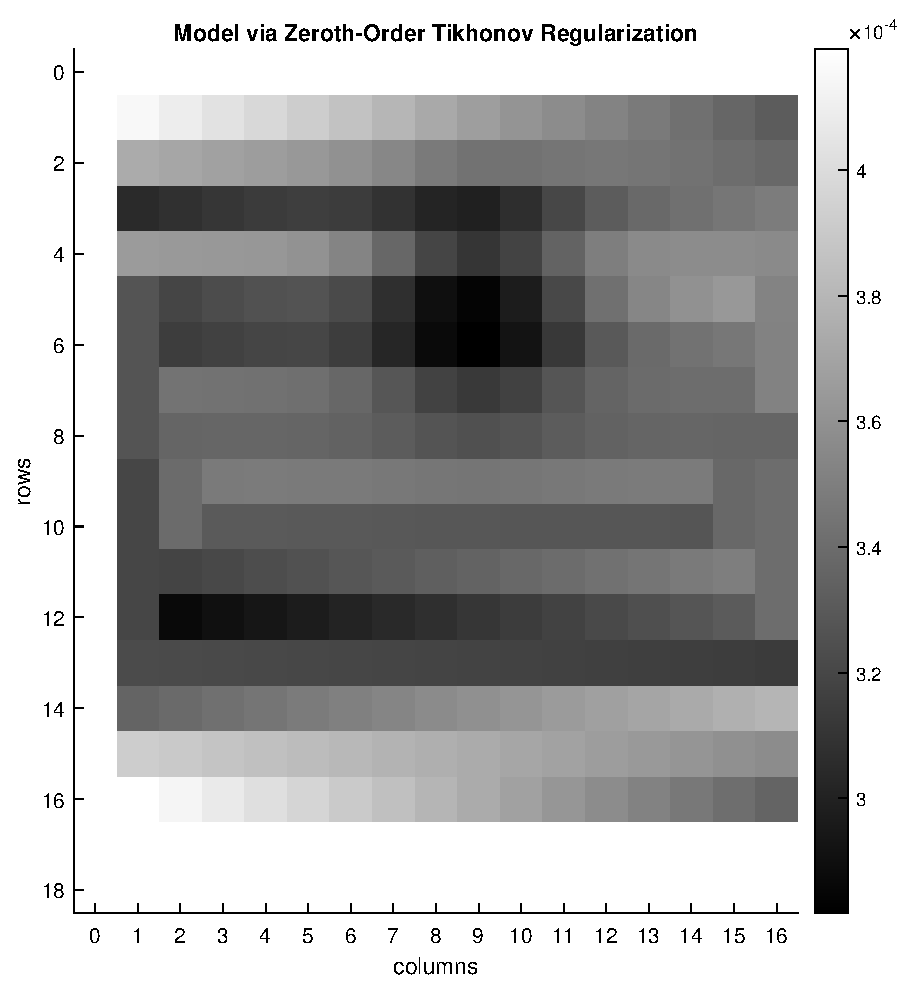
\includegraphics[width=0.85\textwidth]{./images/prob3_partB_m_tikh.eps}
 	\caption{Zeroth-Order Tikhonov Regularization Solution}
 	\label{fig: prob3 partB model}
 \end{figure}
 \FloatBarrier
 
 Using the discrepancy principle is difficult in this situation due to a few reasons. The first common heuristic is to bound the model residuals to the value $\delta < \sqrt{m - n}$, however in our situation $m = n$ which means bounding $\delta$ to zero is unrealistic in the presence of noise. The second heuristic is to simply bound $\delta < m$, however notice that in the L-Curve in figure \ref{fig: prob3 partB L-curve} that all model residuals are below the value $256$, which does not discriminate any potential values in our solution.
 
 
 % Part C
 \subsubsection{Part C - Inverse Problem Solution via Second-Order Tikhonov Regularization}
 
  Again, the L-curve was created using the provided functions \verb*|l_curve_tikh_gsvd()| and \verb*|l_curve_corner()| in the \verb*|PEIP| library. The inputs to the functions used the provided values of $G$ and $\bv{d}$, not their weighted versions. This resulted in the following plot in figure \ref{fig: prob3 partC L-curve}, where the reported value $\alpha = 1.634 \times 10^{-7}$.
 
 \begin{figure}[h] 
 	\centering
 	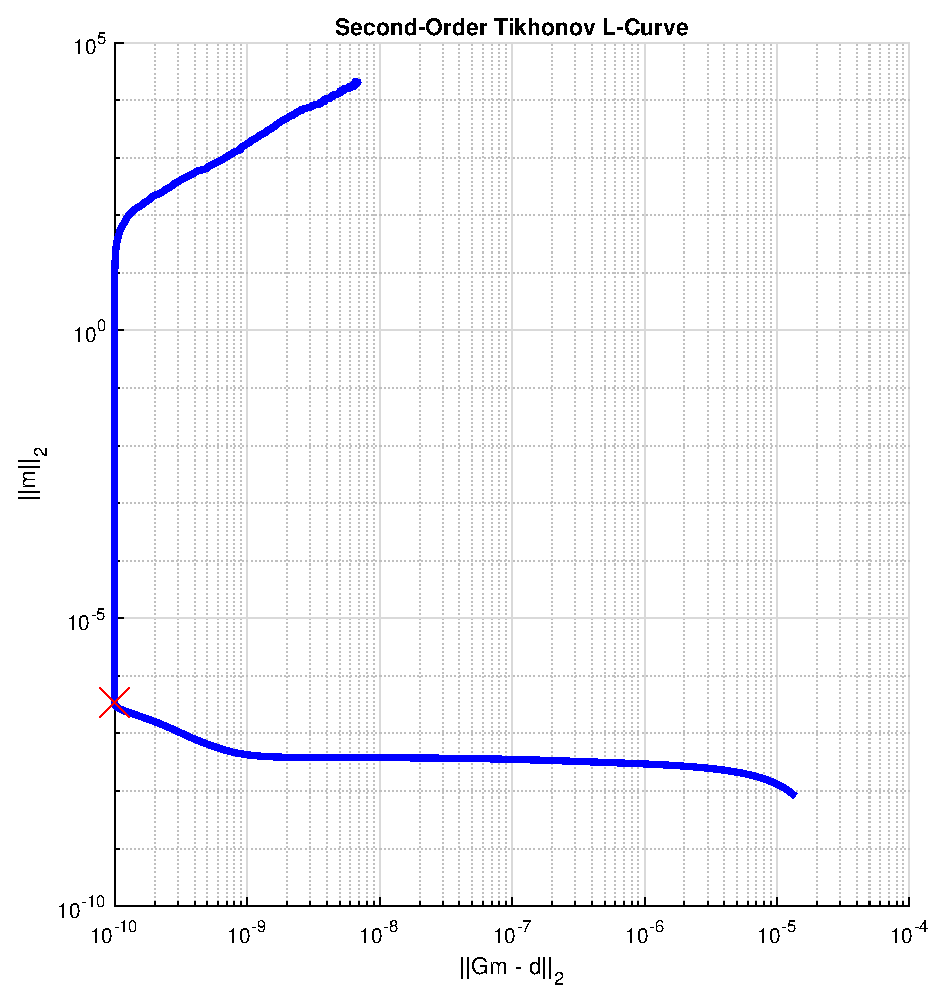
\includegraphics[width=0.85\textwidth]{./images/prob3_partC_tikh_L_Curve.eps}
 	\caption{Second-Order Tikhonov Regularization L-Curve}
 	\label{fig: prob3 partC L-curve}
 \end{figure}
 \FloatBarrier
 
 Notice the curve above is not truly an L-shape as the top of the curve begins tilting into the positive model residual direction. This did not seem to have any impact in selecting the correct corner.
 
The model was solved with the modified normal equations below.

\begin{align*}
	\bv{m}_{tikh,L2} = \left(G_w^T G_w + \alpha^2 L_2^T L_2\right)^{-1} G_w^T \bv{d}
\end{align*}

The result is provided in figure \ref{fig: prob3 partC model}.
 
 \begin{figure}[h] 
 	\centering
 	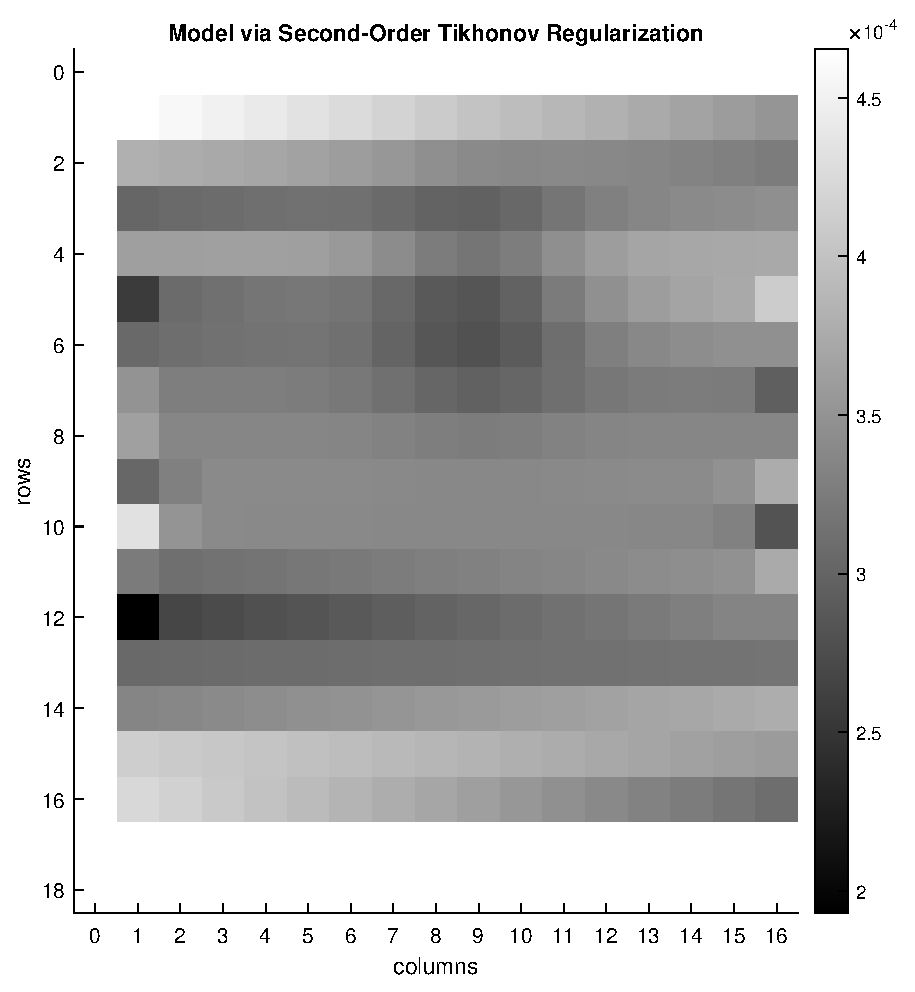
\includegraphics[width=0.85\textwidth]{./images/prob3_partC_m_tikh.eps}
 	\caption{Second-Order Tikhonov Regularization Solution}
 	\label{fig: prob3 partC model}
 \end{figure}
 \FloatBarrier
 

 % Part D
\subsubsection{Part D - Discussion}

Between the three methods, TSVD, Zeroth-Order Tikhonov Regularization, and Second-Order Tikhonov Regularization, each model looks very different from the other. In the TSVD approach, vertical bands do appear within the center 8 blocks especially near the edges. However in the Zeroth-Order approach, horizontal bands appear instead. No bands in either direction appear in the 2nd order approach. The roughing matrix $L_2$ used in Part C consisted of the finite difference for the second derivative in both the row and column directions unlike the other $L_2$ matrix formulations provided in the textbook which likely explains these differences.



